% Paper cover page
\papertitle{A new strategy for matching observed and simulated lensing galaxies}
\capauthors{
    \chapterauthor[1,2]{Philipp Denzel}
    \chapterauthor[3]{Sampath Mukherjee}
    \chapterauthor[2,1]{Prasenjit Saha}
}
\affils{
    \chapteraffil[1]{Institute for Computational Science, University of Zurich, 8057 Zurich, Switzerland}
    \chapteraffil[2]{Physics Institute, University of Zurich, 8057 Zurich, Switzerland}
    \chapteraffil[3]{STAR Institute, Quartier Agora - All\'ee du six Ao$\hat{u}$t, 19c B-4000 Li\`ege, Belgium}
}

%\publishedin[Reference:\\]{}
\clearpage


\newcommand\SDSSJ[1]{\ifthenelse{\equal{#1}{0029}}{\textsc{J0029\textminus0055}}{}\ifthenelse{\equal{#1}{0737}}{\textsc{J0737+3216}}{}\ifthenelse{\equal{#1}{0753}}{\textsc{J0753+3416}}{}\ifthenelse{\equal{#1}{1051}}{\textsc{J1051+4439}}{}\ifthenelse{\equal{#1}{0956}}{\textsc{J0956+5100}}{}\ifthenelse{\equal{#1}{1430}}{\textsc{J1430+6104}}{}\ifthenelse{\equal{#1}{1627}}{\textsc{J1627\textminus0053}}{}\ignorespaces}%
\newcommand\roche{\mathcal{P}}
\renewcommand{\tref}[1]{\hyperlink{tr#1}{(#1)}}
\renewcommand{\tlink}[1]{\hypertarget{tr#1}{(#1)}}



\def\pwidth{.99\textwidth}
\def\qheight{.23\textheight}


% Abstract
\section*{Abstract}
\noindent The study of strong-lensing systems conventionally involves
constructing a mass distribution that can reproduce the observed
multiply-imaging properties.  Such mass reconstructions are
generically non-unique.  Here we present an alternative strategy:
instead of modelling the mass distribution, we search cosmological
galaxy-formation simulations for plausible matches.  In this paper we
test the idea on seven well-studied lenses from the SLACS survey.  For
each of these, we first pre-select a few hundred galaxies from the
EAGLE simulations, using the expected Einstein radius as an initial
criterion.  Then, for each of these pre-selected galaxies, we fit for
the source light distribution, while using MCMC for the placement and
orientation of the lensing galaxy, so as to reproduce the multiple
images and arcs.  The results indicate that the strategy is feasible,
and even yields relative posterior probabilities of two different
galaxy-formation scenarios, though these are not statistically
significant yet.  Extension to other observables, such as kinematics
and colours of the stellar population in the lensing galaxy, is
straightforward in principle, though we have not attempted it yet.
Scaling to arbitrarily large numbers of lenses also appears feasible.
This will be especially relevant for upcoming wide-field surveys,
through which the number of galaxy lenses will rise possibly a
hundredfold, which will overwhelm conventional modelling methods.

\clearpage


% Introduction
%% intro.tex

On May 29, 1919 during a total solar eclipse, three scientists, Eddington,
Dyson, and Davidson, tried to find out what effect, if any, is produced by a
gravitational field on the path of a light ray traversing
it~\cite{Eddington1920}.  During a thoroughly prepared expedition, they measured
the deflection of positions of stars in the previously studied Hyades cluster
caused by the mass of the Sun as predicted by the theory of gravity, general
relativity.  This was the first observation of gravitational lensing, as well as
the first predicted and validated effect of general
relativity~\sidecite{Einstein1911}.

Effectively, gravitational lensing is entirely analogous to optical lenses. In
fact, to produce the distorted light signatures like they are observed in
gravitational lens systems, one only needs a stem from a wine glass and move it
in front of a light source.  A toy example of such a situation can be found
under:
\href{https://phdenzel.github.io/zurich-lens/}{phdenzel.github.io/zurich-lens/}.
In optics, the lens comprises a glass sheet of variable thickness.  It deflects
light by an amount proportional to the local thickness.  The physical process
which causes a change of direction when a ray traverses a glass lens, is called
refraction.  It describes the delay, i.e. decrease in speed of light, due to the
change of media and therefore a change in direction.  While the result of
lensing is the same for both optical and gravitational lenses, the latter causes
the delay and deflection due to the change of the felt gravitational potential
as light moves through it.  The rather rare occurrence of a perfect alignment of
a background source, e.~g. a quasar, and a massive foreground object in which
the imaged source is distorted in a way such that it can be observed multiple
times or even as a ring wrapping around the lens, is called \textit{strong}
gravitational lensing.  \figref{mock-lens} demonstrates such a case with a
mock lens.
\begin{figure}[h]
    \centering
    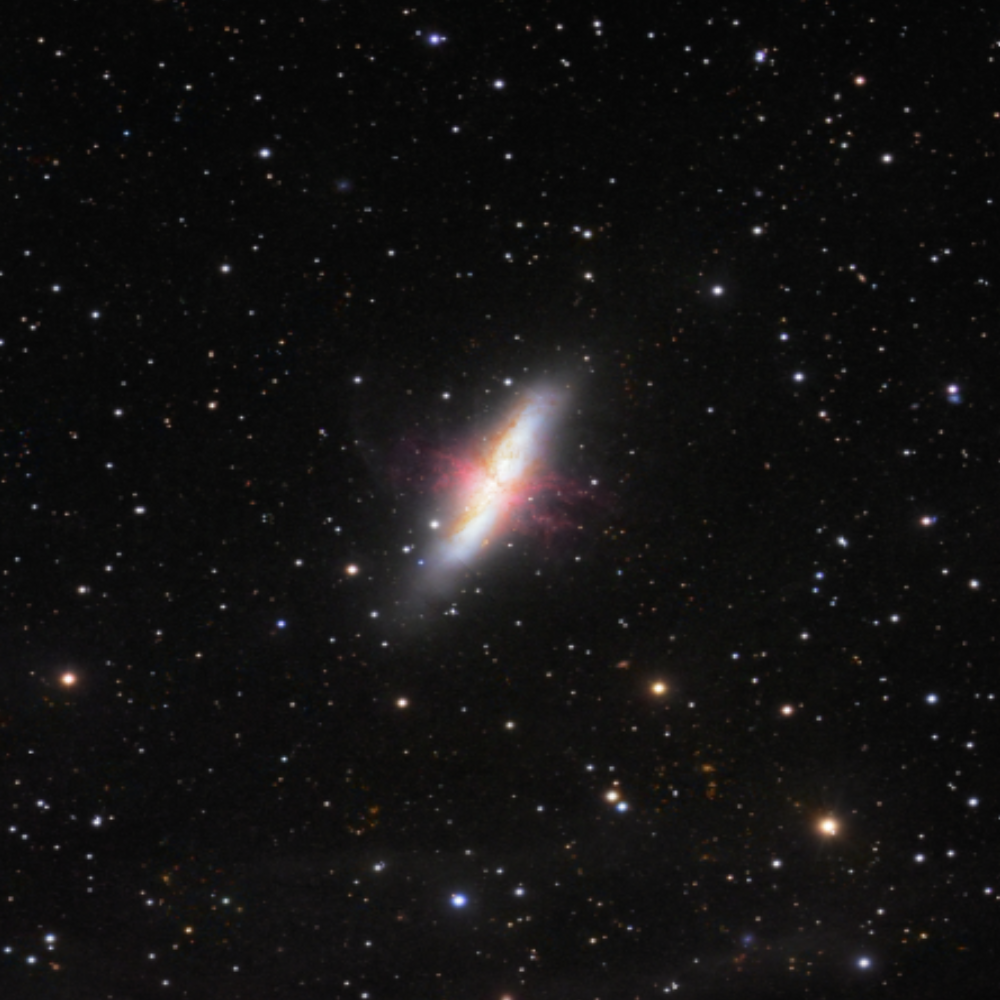
\includegraphics[width=0.49\textwidth]{m82-original}\,%
    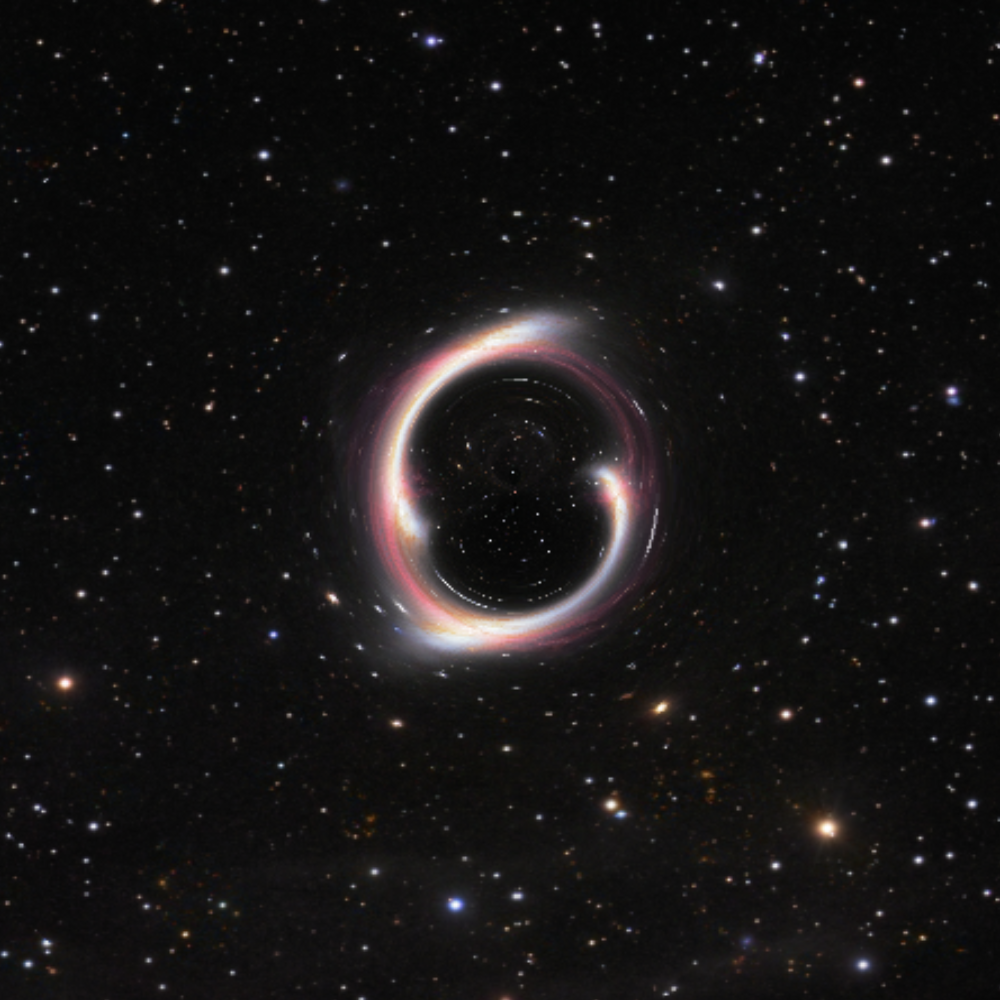
\includegraphics[width=0.49\textwidth]{m82-lensmock}
    \caption[Mock lens image of M82]{Mock lens observation: The left image shows
    the "Cigar Galaxy" M82 cutout from
    \href{https://apod.nasa.gov/apod/ap200515.html}{APOD 2020 May 15}. The right
    image demonstrates what it could look like if for instance a small black
    hole with a third of the Sun's mass would replace the Moon in front of M82.
    The right image was generated using my lens mock code: \Code{lensing.js}
    (\href{https://phdenzel.github.io/lensing.js/}{phdenzel.github.io/lensing.js/}).\\
    \textit{Image Credit \& Copyright: Dietmar Hager, Torsten Grossmann}}
    \figlbl{mock-lens}
\end{figure}

More specifically, the deflection in gravitational lensing is of the order of
$4M/R$, where $M$ is the mass of the lens and $R$ its size.  Strong
gravitational lensing occurs when the apparent size $R/D$ of the aligned lens at
a distance $D$ is comparable to that deflection.  In fact, although the
underlying physical process is all the same, gravitational lensing is
categorized into three types based on the observational techniques and mass or
size regimes: \textit{strong}, \textit{weak}, and \textit{micro} lensing.
\begin{align}
    \text{strong} \hspace{1cm}&\frac{4M}{R} \gtrsim \frac{R}{D}\\
    \text{weak} \hspace{1cm}&\frac{4M}{R} < \frac{R}{D}\\
    \text{micro} \hspace{1cm}&\frac{4M}{R} \gg \frac{R}{D}
\end{align}

\par\noindent\rule{\textwidth}{0.8pt}

Micro lensing is mostly used to

Analysis and research of gravitational lenses\dots

\par\noindent\rule{\textwidth}{0.8pt}

\section{The Expanding Universe}\seclbl{exp_universe}
%% exp_universe.tex

% Discovery of the expanding universe
Like most fundamental theories in physics which helped in the present-time
understanding of our Universe and the interactions within, general relativity
was formulated in the early 20th century.  While the word was spreading of
Einstein's construct of the supposedly quasi-static Universe which involved a
'cosmic constant' to keep it so, Vesto Melvin Slipher and Edwin Hubble performed
the key measurements which provided the connection between theory and
observations.  By 1923, Slipher's hard work yielded a compilation of velocity
estimates for 41 galaxies.  Remarkably, most of those galaxies were receding
from us, and thus appeared redshifted\sidenote{The recession velocity of a
galaxy can be measured by the (Doppler) shift of its spectral lines, i.e.
redshift.}.  Half a decade afterwards, Edwin Hubble investigated the relation
between his distance measurements to these galaxies and their radial velocities.
Thereby, he effectively measured an apparently constant velocity gradient in
units of \Hunitsalt.  This constant was later named after him, the
\textit{Hubble constant}~\Ho.  Through this velocity gradient he realised
something, which could arguably be called the birth of modern cosmology: the
concept of an expanding Universe would explain why all galaxies are receding
from us and each other~\sidecite{Kirshner04,
Hubble1929}\marginnote[0.75cm]{While one would expect such a finding to be
highly cited, Hubble's publication interestingly counts only 73 official
citations at the time of writing.}.  The outward motion of galaxies resulting
from the uniform expansion of the Universe is best observable at very high
distances where the local, mutual gravitational interaction between galaxies is
subdominant.  This behaviour is commonly referred to as the \textit{Hubble
flow}.

Hubble's realisation was an impressive leap of thought, even more so, since the
prevalent idea of the Universe at the time was synonymous to today's picture of
our own galaxy, the Milky Way, beyond which the existence of anything else was
uncertain.  Only around 1920, astronomers started considering that what they
called nebulae were in fact extra-galactic 'island universes' that is entirely
other galaxies.  Today, there are 'standard' recipes for recreating and
improving upon Hubble's results\sidenote{He determined the Hubble constant by
the slope of his iconic diagram with roughly $\Ho \approx 500\,\Hunits{}$.} by
gathering distance and velocity or redshift estimates to galaxies and other
astronomical objects which are much further away.  While this might seem like a
simple task, the matter of measuring distances relates to problems with which
cosmology struggles still today.  

The most 'human' method of measuring distances is the \textit{parallax}.  It
essentially utilises the same principles as the human eye.  With two points of
observation, an astronomical, stereoscopic vision is achieved from which the
distance can be estimated.  However, with even the most sophisticated
technologies reaching high angular resolution, parallax has only very little
reach.  Since the main objective in cosmology is to study the Universe's
large-scale structures from birth to the present, this technique is relatively
ineffective as it rarely reaches objects able to probe the Hubble flow.  Still,
it is generally used as calibration for other techniques with longer reach.  An
especially powerful application of the parallax is the measurement of distances
to galaxies containing megamasers, gas clouds with water molecules which
catalyse the emission of coherent microwave radiation.  Distances to these
emission points can be determined to incredible precision with long baseline
interferometers and spectral monitors.  Another strong influence of the parallax
technique is reflected in the distance unit 'parallax second' which is usually
shortened to \textit{parsec} and ubiquitously employed in astronomy and
astrophysics.  It is the distance where 1 astronomical unit (AU; the nominal
distance of Earth to the Sun) spans 1 arcsecond on the sky.  Using \ref{eq:au}
and \ref{eq:arcsectan}, we can write:
%
\begin{equation}%
    1\,\parsec = 1\,\AU \times \tan(1\,\arcsec)^{-1} \approx 10^{8}\,\lightsec
    \eqlbl{parsec}
\end{equation}%
%
Distance measurements sensitive to the expansion of the Universe have to rely on
different strategies.

In an expanding, flat Universe many different measures of distances can be
defined.  For example, it can be very useful to factor out the expansion and
define the so-called \textit{comoving distance}
%
\begin{equation}\eqlbl{d_comov}%
    d_{comov} = \frac{c}{\Ho} \int_0^{z} \frac{d\zeta}{\sqrt{\Omega_m(1+\zeta)^3
    + \Omega_r(1+\zeta)^4 + \Omega_\Lambda}}.
\end{equation}
%
where $z$ is the redshift of the light to which the distance is measured, and
$\Omega_i=\rho_i/\rho_c$ are the relativistic, non-relativistic, and dark energy
components, normalised by the cosmological critical density $\rho_c$.  Every
component contributes at various scales differently to the expansion or
contraction of the Universe, and therefore have to be considered separately when
distances are measured.  In a flat Universe, the cosmological critical density
is its average density $\propto\Ho{}^{2}/G$.  The comoving distance does not change with time,
assuming the observers are moving with the Hubble flow.  Another measure which
is especially often used in the context of lensing, is the
\textit{angular-diameter distance} which is defined as an object's physical size
over the its angular size as viewed from Earth. It can also be written as
%
\begin{equation}\eqlbl{d_comov}%
    d_{ang} = \frac{d_{comov}}{(1+z)}
\end{equation}
%
It is the distance which freezes the Universe at the time when the light which
is used to measure it, is emitted.  This leads to a very peculiar behaviour that
beyond some redshift the angular-diameter distance actually decreases with
increasing redshift.

For a long time, light from very bright sources represented the only way of
measuring distances in astronomy\sidenote{As explained below, gravitational
waves changed the game in more than one way.}.  Just like lighthouses acted as
distance markers and warning signals for reefs and promontories to mariners
since ancient times, bright light sources called \textit{standard candles}
provide the means for the most common method to determine distances for the
purpose of probing the Hubble flow.  For such objects, the intrinsic luminosity
$L$ can be measured or determined theoretically without measuring their
distance.  By observing their apparent light flux $F$ dimmed by traversing the
vastness of space, a \textit{luminosity distance} can be determined
%
\begin{equation}\eqlbl{d_lum}%
    d_{lum} = \sqrt{\frac{L}{4\pi F}}
\end{equation}%
%
which happens to relate with $d_{lum}={(1+z)\,d_{comov}}$ to the comoving
distance.  Cepheids for instance, variable stars for which the intrinsic
luminosity depends on their periodic behaviour of brightness fluctuations, are
long-known standard candles.  Their luminosity-period relation was discovered by
Henrietta Leavitt in 1912 and enabled the first distance measurements reaching
past the edge of the Milky Way to the Andromeda Galaxy (M31).  The brightest
standard candles known to astronomers however are Type-1a Supernovae (SNeIa).
They are a special variant of Supernova in which a white dwarf in a binary star
system accretes mass.  Due to this process, the exact energy available at the
time of Supernova and thus its standardizable intrinsic luminosity is given by
the Chandrasekhar mass limit of $1.44\mathrm{M_\odot}$.  

Yet withal there is no single method which is applicable to all ranges of
distances.  Thus, a common procedure in the measurement of the Hubble constant
is the \textit{cosmic distance ladder}, in which one distance measurement
iteratively provides calibration for the next, with the end of the rung being
the farthest reaching SNeIa.  Methods based on the distance-redshift relation
are often called 'late' measurements.

Opposed to these are the 'early' measurements, which are based on completely
different physical processes.  Instead of a distance measurement, the 'early'
measurements determine the Hubble constant and other cosmological constants,
with angular modes of temperature on the Cosmic Microwave Background (CMB).  For
instance, the monopole temperature of the CMB evolves with $\dot{T}_{\text{CMB}}
= -\Ho{}T_{\text{CMB}}(t)$.  The current temperature of the CMB is known to be
around $T(0) = 2.725\;\mathrm{K}$. So, with a Hubble constant of the order of
$70\;\Hunitsalt{}$, this yields a change in temperature of roughly
$-0.2\;\mathrm{nK/yr}$ and could be measured with accurate detectors over a long
period of time.  The common method however to infer \Ho{} is based on the
multipole-temperature fluctuations of the CMB.  The particular structure at
angular sizes in the CMB arises due to baryonic acoustic oscillations (BAO)
which are an imprint of pressure waves in the primordial baryon-photon plasma.
Therefore, the amplitudes of the BAO peaks depend on the baryon-density
component of the Universe through which the Hubble constant can be indirectly
determined.  Such methods obtain estimates which are independent of the cosmic
distance ladder employed by 'late'-Universe measurements.

The separation between 'early' and 'late' measurements of the Hubble constant
has been emphasised in the last decade, because of a discrepancy in the results
they yielded.  While measurements of late-Universe probes indicate a Hubble
constant of around $\Ho = 74.0 \pm 1.4\;\Hunitsalt$~\sidecite[][latest results
obtained by the SH0ES (Supernovae \Ho\ for the Equation of State) project which
measures the Hubble constant using Supernovae]{Riess19}, 'early'-Universe
measurements generally yield a lower value of $\Ho = 67.4 \pm
0.5\;\Hunitsalt$~\sidecite[][most recent inference of the cosmological
parameters from the Planck collaboration]{Planck18b}.  In the comparison of the
values and uncertainties of such determinations, it becomes apparent that there
is a discrepancy at a $4.5\sigma-5.5\sigma$-level\sidenote{depending on the
exact measurements being compared} between these two opposing sides.  This means
that there is roughly a 1 in 20'000'000 chance of both measurements being
different on accident, which indicates a problem with either one or both
methods.  The seemingly only way to resolve this so-called \textit{Hubble
tension}, without completely changing the concordance model of cosmology, is to
find some so-far unknown systematic errors in the measurements which would
account for the discrepancies.  As it currently stands however, the Hubble
tension appears to force the rejection of the most successful cosmological
concordance model, the $\Lambda$ cold-dark matter model ($\Lambda$CDM). 

For this reason, it is crucial to have as many independent methods of obtaining
estimates for the Hubble constant as possible, each with sufficient precision to
resolve the tension.  In the past couple of years, gravitational lenses were
believed to provide a third perspective on the issue and possibly resolve the
discrepancies surrounding the value of \Ho{}.  While other methods are based on
standardizable luminosity measurements or the angular power spectrum of the CMB,
gravitational lenses induce differences in travel times of light rays, so-called
time delays, which can be measured in the lensed images of quasars and other
time-variable sources over a period of the order of years.  These time delays
set the scale of the lensing system and are proportional to the inverse of the
Hubble constant, the Hubble time.  Through these time delays, the recovery of
the lensing-mass distribution therefore allows an independent measurement of the
Hubble constant from a completely different physical process.  

\chref{delays} presents a critical study of such a measurement.  With an
analysis on 8 time-delay lenses, I determined the Hubble constant with a value
of \sidenote{\protect\textcolor{red}{TODO}: I was told that one should use 'I'
in the intro... is this really what is usually done?}
%
\begin{equation*}%
    \Ho = 71.8^{+3.8}_{-3.3}\;\Hunitsalt
\end{equation*}%
%
The value is compatible with both the early and late measurements, with a
tension of less than $1.5\sigma$.  With a precision of 4.9\%, the measurement is
unfortunately not able to contribute to the resolution of the Hubble tension.
In fact, the investigation revealed that, if a 1\% level is at all obtainable,
it would require a joint-analysis of many more time-delay measurements of
quadruply imaging lens systems (quads).  It was not the only determination of
the Hubble constant through lensing observations recently; the H0LiCOW
collaboration \sidecite{Wong19} reported on a Hubble constant of
$73.3^{+1.7}_{-1.8}\;\Hunitsalt$ from 6 time-delay lenses a year before, and the
STRIDES collaboration \sidecite{Shajib20} determined a value of
$74.2^{+2.7}_{-3.0}\;\Hunitsalt$ from a single lens.  However, while these
results were reported with higher confidence, this study explores many different
lens models and thus accounts for lensing degeneracies by construction.
Although degeneracies are often neglected in lensing studies, it is known for a
long time that a family of lens-mass distributions is able reproduce the same
observables, but still yield different values for the Hubble constant.
Therefore, studies with the aim of inferring the Hubble constant need to solve
for (ideally) all possible solutions of mass distributions in order to retrieve
a complete model.  The study produced 8000 lens-mass distributions with 1000
values for the Hubble constant.  Most interestingly, the values appeared to be
asymmetrically distributed, which might indicate that the errors on \Ho{} could
be non-Gaussian.  These results were not entirely unexpected since the
investigation was actually a continuation of ideas gathered during a
participation in a scientific blind study \sidecite{TDLMC2} in which 50
simulated time-delay lenses were analysed by several research groups.  It
discovered that current lens recovery methods are accurate to only about 6\%,
even with acclaimed precision over nearly 1\%.  In comparison with the study
presented in \chref{delays}, it became apparent that the lens simulations
considerably differed from real observations and that the uncertainties in the
inference of \Ho{} from mock lenses were higher.  Besides the obvious numerical
deviations, the radial distribution of lens images of the simulated lens set was
relatively narrow which provided only little constraints on the slope of the
density profile and consequently on \Ho.  This could mean that there exists a
limit to the accuracy on \Ho{} achievable with time-delay galaxy lenses, which
ultimately might preclude them to infer \Ho{} on a level required to resolve the
Hubble tension.  Nonetheless, gravitational lenses are excellent cosmological
probes. Especially cluster lenses do not exhibit this limitation and might still
recover the Hubble constant with sufficient precision to contribute to the
resolution of the Hubble tension.

Even so, it is unlikely for a single method to resolve the Hubble tension alone.
However, another promising approach to determine distances has emerged.  Light
signals weaken with the square of their distance as described by \eqref{d_lum}.
This means a signal will be 4 times less bright at twice the distance, which is
generally the case for long-range physical laws, be it the gravitational force,
electro-magnetic force, or most kinds of radiation.  Of course, for a constant
progress out into the cosmos, the demand on technologies is twice as high and
pushes them to their limits.  Recently however, the detection of gravitational
waves changed the game.  When two massive, compact objects such as black holes
orbit each other and start to inspiral, some amount of energy is emitted in form
of gravitational waves\sidenote{a highly non-classical effect!}.  A major
advantage over their electro-magnetic counterpart is that the signal strength of
gravitational waves decreases with distance linearly.  The benefits of this
become immediately apparent: if one would manage to build a detector which is
100 times as sensitive, it could measure distances 100 times as far into the
Universe, rather than 10 times as far with a light detector which was 100 times
as sensitive.  The reason for the linear dependence on distance lies in the
method how the signal is generated and measured.  The easiest way of generating
electro-magnetic waves is to move charges back and forth which creates dipole
radiation, commonly known as light.  Due to the conservation of momentum, this
is not possible for gravitational waves which instead consist of quadrupole
radiation.  These kinds of radiations are fundamentally different when it comes
to their detection.  While light simply gets absorbed in the detector and
changes the energy level of the detected signal, gravitational waves induce
stretching and compression in the detector, called strain which is proportional
to the amplitude of the wave.  While the energy of gravitational waves still
falls with the square of the distance, their amplitude decrease with the
distance linearly, which is ultimately the reason of the farther reach of
distance measurements based on gravitational waves.  In the future, this method
of measuring distances will be crucial in resolving the discrepancies in the
measurements of the Hubble constant.


\section{The Solar Neighbourhood}\seclbl{solar_nbhood}
%% solar_nbhood.tex

Even within the Milky Way, measuring velocities and distances was and still is a
complicated endeavour.  Earth is revolving around our Sun, and the Solar System
is orbiting around the Galactic center, which means relative motions have to be
carefully examined.  From some locations on Earth, a dense strip of starlight is
visible across the night sky which is indicative of the Galaxy's disk structure.

\begin{figure}[h]
    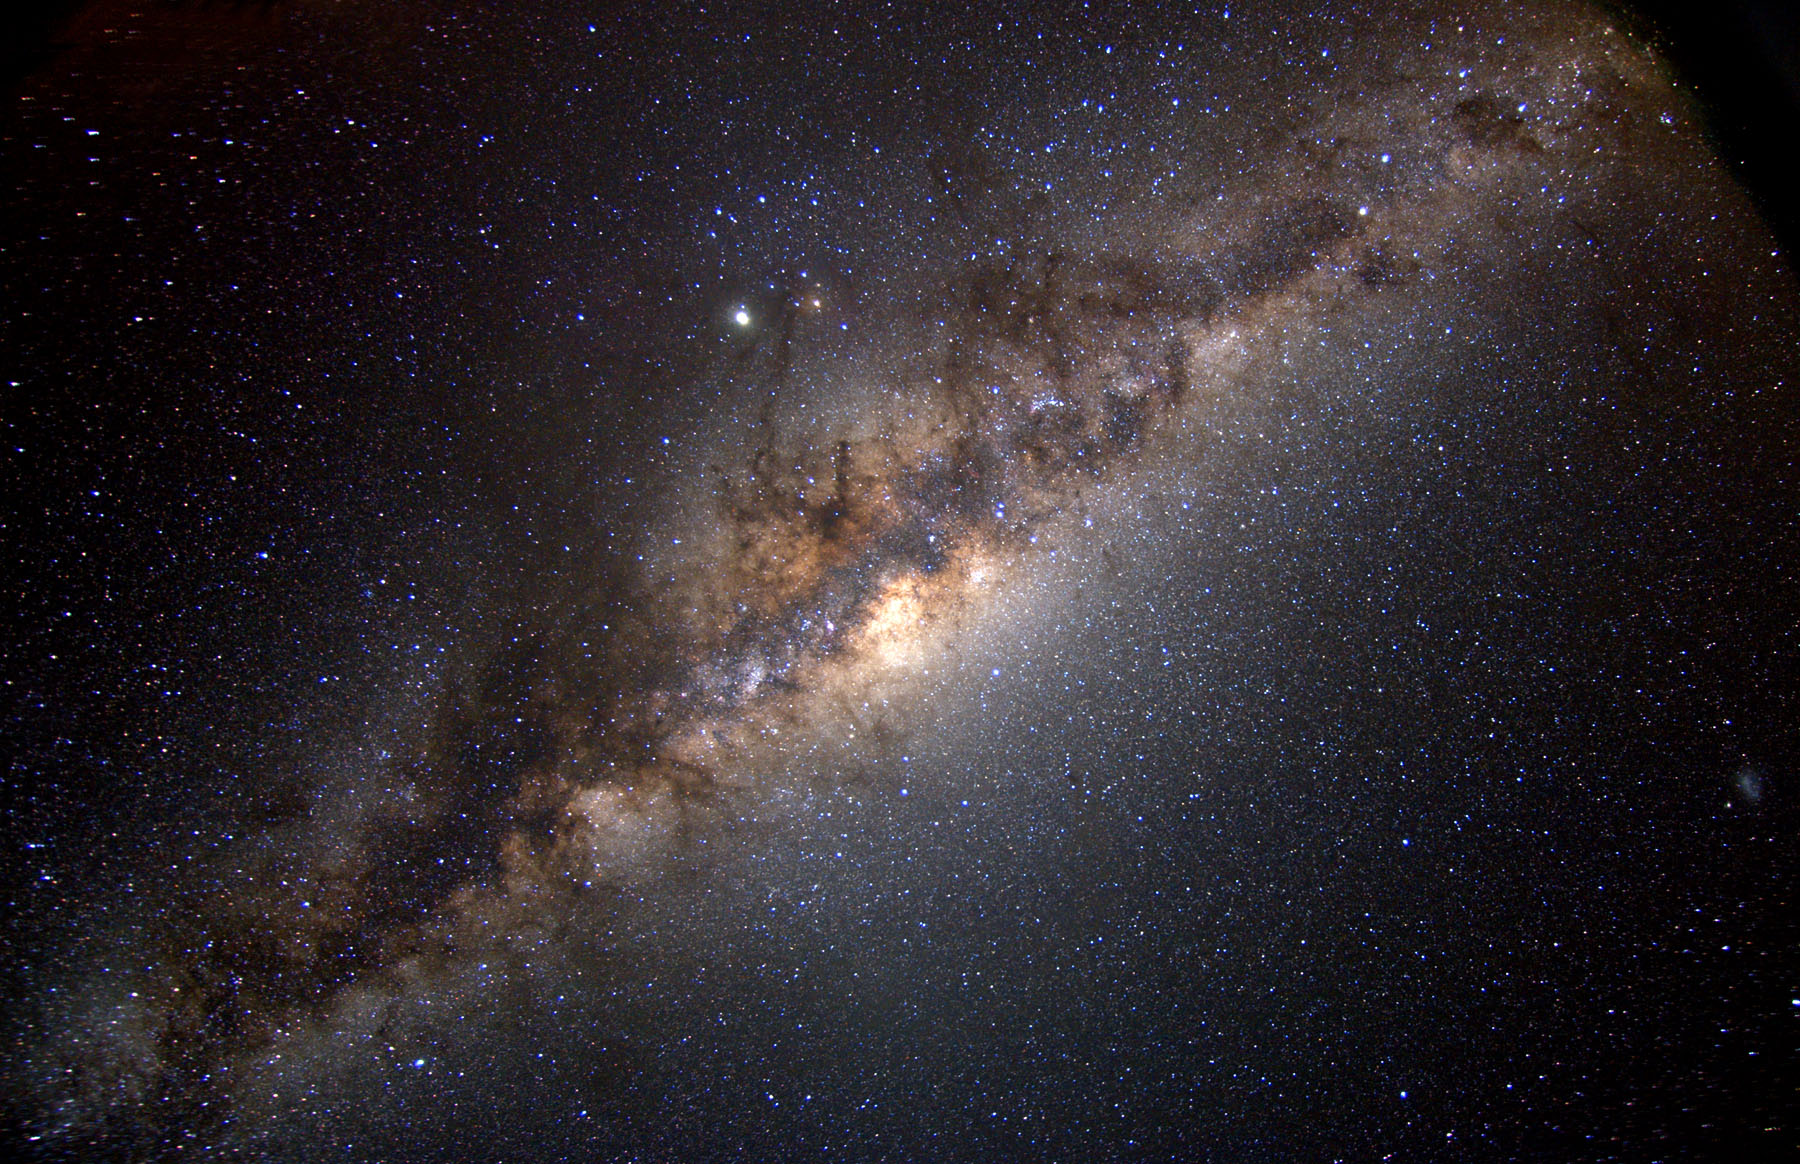
\includegraphics{apod080104}
    \caption[The Milky Way: APOD 2008 January
    4]{\href{https://apod.nasa.gov/apod/ap080104.html}{APOD 2008 January 4}: The
    Milky Way at 5000 meters.\\
    View on our own galaxy from within (recorded in the Chilean Andes).  The
    band of the dense collection of stars from the disk and the Galactic center
    is partially covered by the typical extinction features due to dust
    clouds.  This suggest that the Milky Way possesses a stellar disk.\\
    \textit{Credit \& Copyright: Serge Brunier}}
    \figlbl{milkyway}
\end{figure}

From far away it is quite easy to recognize the typical morphology of other
galaxies through direct observations\sidenote{Provided the telescope has enough
angular resolution.}.  Measuring their rotational properties already becomes
increasingly difficult, deducing the shape and rotation patterns of the Milky
Way from within however is an undertaking of its own.

A possibly random and dense distribution of stars as it appears in galaxies
should in principle collapse towards its potential well.  Like in many other
astrophysical scenarii, pressure gradients can take a stabilizing role and
balance gravity.  These balancing pressures depend on different physical
processes and generally define limiting scales.  For some galaxies, e.g.
ellipticals, the stars' random motions are the dominant drivers towards
stability, for spiral galaxies it is their rotation about the disk's center.  In
contrast to orbiting systems such as the Sun and Earth, where most of the mass
is located near the guiding center of the orbits, the Milky Way's mass
distribution is more complex with different elements such as various forms of
hydrogen gas, dust, stars, and stellar remnants.  In general, the study of
galactic rotation through stars can yield insights not only into the galaxy's
morphology, but also into its formation history and mass composition.  One of
the most powerful tools therefor is the rotation curve $V(R)$.  It characterizes
the orbital velocity as a function of distance from the Galactic center. By
measuring how $V(R)$ behaves with radius, we can draw conclusions about the
Milky Way's size, total mass, and the distribution thereof.  A solid-body
rotation $V \propto R$ would mean that the enclosed mass ideally increases with
$R^{2}$, Keplerian orbits go as $V \propto R^{-\half}$, whereas $V \propto
\text{const.}$ is a result of the enclosed mass increasing as $R$.

Milky Way's rotation curve can be probed through its stars. Prime observable is
the radial velocity $v_{r}$, and in principle the tangential velocity $v_{t}$,
distance from Earth $d$ and longitude on the sky $l$ too.  Measurements of these
quantities can be combined to the so-called \textit{Oort's constants}
\begin{align}
    &A = \frac{v_{r}}{d\sin{2l}} \hspace{0.5cm}\nonumber\\[5pt]%
    &B = \frac{v_{t}}{d} - A\cos{2l}.
    \eqlbl{obs_oortsC}
\end{align}

A caveat is the assumption that the stars, including the Sun, are on circular
orbits, which is only approximately true.  Moreover, it assumes the Milky Way
has a monotonically decreasing, symmetric potential.  Again, this is not
entirely true as spiral arms can introduce over-densities which manifest as
asymmetries and locally break monotonic behaviour in the potential.  Still,
within their limits the Oort's constants are very useful, because they can be
rewritten as
\begin{align}
    &A = -\frac{1}{2} \left[\frac{\derivd V}{\derivd R} - \frac{V_{0}}{R_{0}}\right]\nonumber\\[5pt]%
    &B = -\frac{1}{2}\left[\frac{V_{0}}{R_{0}} + \frac{\derivd V}{\derivd R}\right].
    \eqlbl{oortsC}
\end{align}

These constants express the shear and vorticity of the disk in the solar
neighbourhood.  The shear essentially measures a deviation from solid-body
rotation, the vorticity how the angular momentum varies with small changes in
radius.  Adding both $A+B = -\frac{\derivd V}{\derivd R}$

\section{Number of lensing galaxies}\seclbl{number_lenses}
%% number_lenses.tex

Put a galaxy similar to MW at half the distance to the 
  
% Methods
\input{\home/tex/methods.tex}

% SEAGLE
\input{\home/tex/seagle.tex}

% Test cases
\input{\home/tex/testcases.tex}

% Results
\input{\home/tex/results.tex}

% Conclusion
\input{\home/tex/conclusion.tex}


%%%% Acknowledgements
\section*{Acknowledgments}

  We would like to thank Liliya L. R. Williams and Dominique Sluse for useful
  discussions and suggestions on how to improve this paper.

  % We also thank the anonymous referee for the constructive suggestions to
  % bring the paper to its final form.

  PD acknowledges support from the Swiss National Science Foundation.  SM
  acknowledges the funding from the European Research Council (ERC) under the
  EUs Horizon 2020 research and innovation programme (COSMICLENS; grant
  agreement no. 787886).

  This research is based on observations made with the NASA/ESA Hubble Space
  Telescope obtained from the Space Telescope Science Institute, which is
  operated by the Association of Universities for Research in Astronomy, Inc.,
  under NASA contract NAS 5–26555. These observations are associated with
  programs \#10886, \#10174, \#12210, \#10494.

\section*{Data availability}
  The data underlying this article are available at the STScI
  (\href{https://mast.stsci.edu/}{https://mast.stsci.edu/}; the unique
  identifiers are cited in the acknowledgements).  The derived data generated in
  this research will be shared on request to the corresponding author, or can be
  replicated using the open-source software available at:
  \faGithub\;\href{https://github.com/phdenzel/gleam}{https://github.com/phdenzel/gleam}.


% Figures
\input{\home/fig/figures}